\newpage
\section{贝叶斯分类器}
\subsection{贝叶斯决策论(Bayesian decision theory)}
假设有 $N$ 种可能的类别标记, i.e. $\mathcal{Y}=\{ c_1,c_2,\dots,c_N \}$, $\lambda_{ij}$ 是将一个真实标记为 $c_j$ 的样本误分类为 $c_i$ 所产生的损失, 基于后验概率 $P(c_i|\bx)$ 可获得将样本 $\bx$ 分类为 $c_i$ 所产生的期望损失, 即样本 $\bx$ 上的条件风险
\begin{align*}
    R(c_i|\bx)=\sum_{j=1}^N\lambda_{ij}P(c_j|\bx)
\end{align*}
任务是寻找一个判定准则 $h:\mathcal{X}\mapsto\mathcal{Y}$ 以最小化总体风险
\begin{align*}
    R(h)=\mathbb{E}_{\bx}\left[ R(h(\bx)|\bx) \right]
\end{align*}
根据贝叶斯判定准则(Bayes decision rule):为最小化总体风险,只需在每个样本上选择那个能使条件风险$R(c|\bx)$最小的类别标记,即
\begin{align*}
    h^*(\bx)=\argmin_{c\in\mathcal{Y}}R(c|\bx)
\end{align*}
此时 $h^*$ 称为 贝叶斯最优分类器(Bayes optimal classifier),与之对应的总体风
险 $R(h^*)$ 称为贝叶斯风险(Bayes risk). $1-R(h^*)$ 反映了分类器所能达到的最
好性能,即通过机器学习所能产生的模型精度的理论上限.

\subsubsection{判别式 vs. 生成式}
欲使用贝叶斯判定准则来最小化决策风险,首先要获得后验概率 $P ( c | \bx)$. 
\begin{itemize}
    \item 判别式: 直接对 $P(c|\bm x)$ 建模
    \item 生成式: 先对 $P(\bm x,c)$ 建模, 再获得 $\displaystyle P(c|\bm x)=\frac{P(\bm x, c)}{P(\bm x)}$
\end{itemize}

\subsubsection{贝叶斯定理}
基于贝叶斯定理, $P(c|\bx)$ 可写为
\begin{align*}
    P(c|\bx)=\frac{P(c)P(\bx|c)}{P(\bx)}
\end{align*}
其中,$P ( c )$ 是 类 “先验”(prior)概率;  $P ( \bx | c )$ 是 样 本 $\bx$ 相 对 于 类 标 记 $c$ 的类 条件概率(class-conditional probability),或 称 为 “似然" (likelihood); $P(\bx)$是 用 于 归 一 化 的 “证 据 " (evidence)因 子 .对 给 定 样 本 $\bx$ 证 据 因 子$ P (\bx ) $与类标 记无关,因此估 计 $P ( c |\bx) $的 问题就转化为如何基于训练数据 $D$ 来估计先验 $P ( c )$ 和似然 $P (\bx | c)$.
\subsubsection{极大似然估计}
先假设某种概率分布形式,再基于训练样例对参数进行估计. 估计结果的准确性严重依赖于所假设的概率分布形式是否符合潜在的真实分布

假定 $P(\bx|c)$ 具有确定的形式并且被参数向量 $\bm{\theta}_c$ 唯一确定, 任务就是利用训练集 $D$ 估计参数 $\bm{\theta}_c$, i.e. 估计 $P(\bx|\bm{\theta}_c)$ 作为 $P(\bx|c)$ 使用. 

令 $D_c$ 表示训练集 $D$ 种第 $c$ 类样本组成的集合, 假设样本独立同分布, 则参数 $\bm{\theta}_c$ 对训练集 $D_c$ 的似然是
\begin{align*}
    P(D_c| \bm{\theta}_c)=\prod_{\bx\in D_c}P(\bx|\bm{\theta}_c)
\end{align*}
其对数似然
\begin{align*}
    LL(\bm{\theta}_c)&=\log P(D_c|\bm{\theta}_c)\\
    &=\sum_{\bx\in D_c}\log P(\bx|\bm{\theta}_c)
\end{align*}
$\bm{\theta}_c$ 的极大似然估计$\hat{\bm{\theta}}_c$为
\begin{align*}
    \hat{\bm{\theta}}_c=\argmin_{\bm{\theta}_c}LL(\bm{\theta}_c)
\end{align*}


\subsection{朴素贝叶斯分类器}
“属性条件独立性假设 " (attribute conditional independence assumption): 对
已知类别,假设所有属性相互独立.换言之,假设每个属性独立地对分类结果发
生影响. 基于此, 有
\begin{align*}
    P(c|\bx)=\frac{P(c)P(\bx|c)}{P(\bx)}=\frac{P(c)}{P(\bx)}\prod_{i=1}^dP(x_i|c)
\end{align*}
其 中 $d$ 为属性数目,$x_i$ 为 $\bx$ 在 第 $i$ 个属性上的取值.

由于对所有类别来说$P (\bx )$ 相同,因此贝叶斯判定准则有
\begin{align*}
    h_{nb}(\bx)=\argmin_{c\in\mathcal{Y}}P(c)\prod_{i=1}^d P(x_i|c)
\end{align*}

估计出类先验概率
\begin{align*}
    P(c)=\frac{|D_c|}{|D|}
\end{align*}

对离散属性而言, 令 $D_{c, x_i}$ 表示 $D_c$ 中在第 $i$ 个属性上取值为 $x_i$ 的样本组成的集合, 则条件概率 $P(x_i|c)$ 可估计为
\begin{align*}
    P(x_i|c)=\frac{|D_{c,x_i}|}{|D_c|}
\end{align*}

对连续属性可考虑概率密度函数, 假定
\begin{align*}
    p(x_i|c)\sim \mathcal{N}(\mu_{c,i}, \sigma_{c,i}^2)
\end{align*}
求出 $\mu_{c,i}$, $\sigma_{c,i}$ 即可知其分布. 
\subsubsection{拉普拉斯修正 (Laplacian correction)}
若某个属性值在训练集中没有与某个类同时出现过,则直接计算会出现问题,因为概率连乘将“抹去”其他属性提供的信息. 

令 $N$ 表示训练集 $D$ 中可能的类别数, $N_i$ 表示第 $i$ 个属性可能的取值数, 修正式为
\begin{align*}
    \hat{P}(c)&=\frac{|D_c|+1}{|D|+N}\\
    \hat{P}(x_i|c)&=\frac{|D_{c,x_i}|+1}{|D_c|+N_i}
\end{align*}
假设了属性值与类别的均匀分布,这是额外引入的 bias. 

\subsection{半朴素贝叶斯分类器 (semi-naïve Bayes classifier)}
基本思路:适当考虑一部分属性间的相互依赖信息. 

最常用策略:独依赖估计 (One-Dependent Estimator, ODE), 假设每个属性在类别之外最多仅依赖一个其他属性
\begin{align*}
    P(c|\bx)\propto P(c)\prod_{i=1}^d P(x_i|c, pa_i)
\end{align*}
其 中 $p a_i$ 为属性 $x_i$ 所依赖的属性,称 为 $x_i$ 的 父 属 性. 

确定每个属性的父属性有几种常见方法:
\begin{itemize}
    \item SPODE (Super-Parent ODE)
    \subitem 假设所有属性都依赖于同一属性,称为``超父'' (Super-Parent),然后通过交叉验证等模型选择方法来确定超父属性
    \item TAN (Tree Augmented naïve Bayes)
    \subitem 以属性间的条件``互信息''(mutual information)为边的权重,构建完全图,再利用最大带权生成树算法,仅保留强相关属性间的依赖性
    \item AODE  (Averaged One-Dependent Estimator)
    \subitem 尝试将每个属性作为超父来构建SPODE ,然后将那些具有足够训练数据支撑的SPODE集成起来作为最终结果,
\end{itemize}

\begin{figure}[!htb]
    \centering
    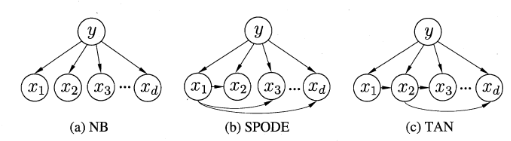
\includegraphics[width=0.42\textwidth]{pic/ML6/朴素贝叶斯与两种半朴素贝叶斯分类器所考虑的属性依赖关系}
    \caption{朴素贝叶斯与两种半朴素贝叶斯分类器所考虑的属性依赖关系}
\end{figure}

\subsection{贝叶斯网(Bayesian network)}
贝叶斯网(Bayesian network)亦 称 “信念网”(belief network),它借助有向
无 环 图 (Directed Acyclic Graph ,简 称 DAG)来刻画属性之间的依赖关系,并使用条件概率表(Conditional Probability Table,简 称 CPT)来描述属性的联合概
率分布.

一个贝叶斯网 $B$ 由结构$G$ 和 参数$\Theta$ 两部分构成,即 $B=(G, \Theta)$. 参 数 $\Theta$ 定量描述这种依赖关系, 假 设 属 性 $x_i$ 在 $G$ 中 的 父 结 点 集 为 $\pi_i$, 则 $\Theta$ 包含了每个属性的条件概率表 $\theta_{x_i|\pi_i}=P_B(x_i|\pi_i)$

给定父结点集,贝叶斯网假设每个属性与其非后裔属性独立

\subsubsection{结构}
\subsubsection{学习}
\subsubsection{推断}
近似推断: 吉布斯采样

进行 $T$ 次采样,每次采样中逐个考察每个非证据变量:假定所有
其他属性取当前值,推断出采样概率,然后根据该概率采样

\subsection{EM 算法}
未 观 测 变 量 的 学 名 是 “隐变量" (latent variable). EM (Expectation-Maximization)算 法是常用的估计参数隐变量的利器. 

令 $\bm X$ 表示已观测变量集,$\bm Z$ 表示隐变量集,$\Theta$ 表 示模型参数.若欲对 $\Theta$ 做极大似然估计,则应最大化对数似然
\begin{align*}
    LL(\Theta|\bm X,\bm Z)=\ln P(\bm X, \bm Z |\Theta)
\end{align*}
通过对Z 计算期望,来最大化已观测数据的对数“边 际 似 然 "(marginal likelihood)
\begin{align*}
    LL(\Theta|\bm X)=\ln P(\bm X|\Theta)=\ln \sum_{\bm Z}P(\bm X, \bm Z|\Theta)
\end{align*}

以初始值$\Theta^0$ 为起点,对其可迭代执行以下步骤直至收敛
\begin{enumerate}
    \item  基于$\Theta^t$ 推 断 隐 变 量 $\bm Z$ 的期望,记 为 $\bm Z^t$
    \item 基于已观测变量 $\bm X$ 和 $\bm Z^t$ 对 参 数 $\Theta$ 做极大似然估计,记 为 $\Theta^{t+1}$
\end{enumerate}

进一步, 不是取 $\bm Z$ 的期望, 而是基于 $\Theta^t$ 计算隐变量 $\bm Z$ 的概率分布 $P(\bm Z| \bm X, \Theta^t)$, 则 EM  的两步为:
\begin{enumerate}
    \item E 步: 以当前参数 $\Theta^t$ 推断隐变量分布 $P(\bm Z| \bm X, \Theta^t)$, 并计算对数似然 $LL(\Theta|\bm X, \bm Z)$ 关于 $\bm Z$ 的期望
    \begin{align*}
        Q(\Theta|\Theta^t)=\mathbb{E}_{\bm Z|\bm X,\Theta^t}LL(\Theta|\bm X, \bm Z)
    \end{align*}
    \item M 步: :寻找参数最大化期望似然,即
    \begin{align*}
        \Theta^{t+1}=\argmax_{\Theta}Q(\Theta|\Theta^t)
    \end{align*}
\end{enumerate}